\documentclass[10pt]{article}
\usepackage[T1]{fontenc}
\usepackage[margin=0.9in]{geometry}
\usepackage{lmodern,microtype,amsmath,amssymb,booktabs,tabularx,graphicx}
\usepackage[numbers,sort&compress]{natbib}
\renewcommand{\bibfont}{\footnotesize}\setlength{\bibsep}{3pt}
\usepackage{xcolor,tikz,xurl}
\usetikzlibrary{arrows.meta,positioning}
\usepackage[hidelinks]{hyperref}
\definecolor{ink}{HTML}{273747}
\setlength{\emergencystretch}{2em}
\setlength{\textfloatsep}{12pt plus 3pt minus 3pt}
\title{Robogogogo: A Tabletop Simulation Workbench\\for Object Collection and Policy Integration}
\author{the Robo Team}
\date{November 27, 2026}
\hypersetup{pdftitle={Robogogogo: A Tabletop Simulation Workbench for Object Collection and Policy Integration},pdfauthor={the Robo Team}}

\begin{document}
\maketitle
\begin{abstract}
Familiar objects provide a concrete setting for examining how robot observations, actions, and task outcomes are represented in a simulation environment. We describe Robogogogo, a local tabletop workbench combining a simulated Franka Emika Panda with eight textured scans from the Yale--CMU--Berkeley object set. Objects retain metric geometry and are represented as independent rigid bodies with approximate collision models. Users can manipulate one object or select a named target among several objects and collect it into a designated cell. The environment couples explicit simulation stepping, manual control, and a scripted reference controller with temporally aligned observations and action records. Stored physical states support replay of the complete scene, while a separate policy interface supplies task instructions, camera images, and proprioception for future vision--language--action integration. An illustrative sequence collects all eight objects without resetting their physical state between targets. This paper documents the environment design and the scope of that demonstration; learned perception, policy generalization, and physical transfer remain questions for subsequent study.
\end{abstract}
\noindent\textbf{Keywords:} robot simulation; object collection; demonstration data; vision--language--action; world models.

\section{Introduction}
A useful robot simulation workbench should connect recognizable objects to physical interactions that can be inspected, repeated, and recorded. For tabletop manipulation, this means more than displaying a textured mesh: the object must have a defined scale, collision geometry, and dynamics, and the recorded action must describe the command that produced the next observation. This relationship matters when the same environment is used first for interactive exploration and later as an interface to a learned policy.

Robogogogo~\cite{robogogogo} develops this workflow around one Panda arm and a small collection of scanned household objects, fruit, and a toy. A user can load the objects together, choose a target by name, and execute a physical grasp-and-place sequence while the remaining objects stay in the scene. A dedicated collection cell for each object permits successive tasks without restoring the initial arrangement. Figure~\ref{fig:tabletop} shows a recorded lemon grasp among the other objects.

The motivation is a compact, inspectable environment for object interaction and demonstration collection. Established engines, asset libraries, and robot-learning platforms already provide much of the underlying functionality. Our account therefore concerns how these components are assembled into this workbench, how an episode is defined when targets change within a persistent scene, and where the interface to a future vision--language--action (VLA) policy lies.

The present task uses known scene identities and positions to direct a scripted controller. Choosing the word ``lemon'' in the interface identifies an object instance; it is not a visual recognition result. The policy interface is deliberately narrower: it exposes the instruction, robot observations, and optional images, with object poses reserved for task accounting and the reference controller. This separation allows a later learned policy to act through the same dynamics without inheriting the demonstrator's object-state access.

\begin{figure}[!htbp]
\centering
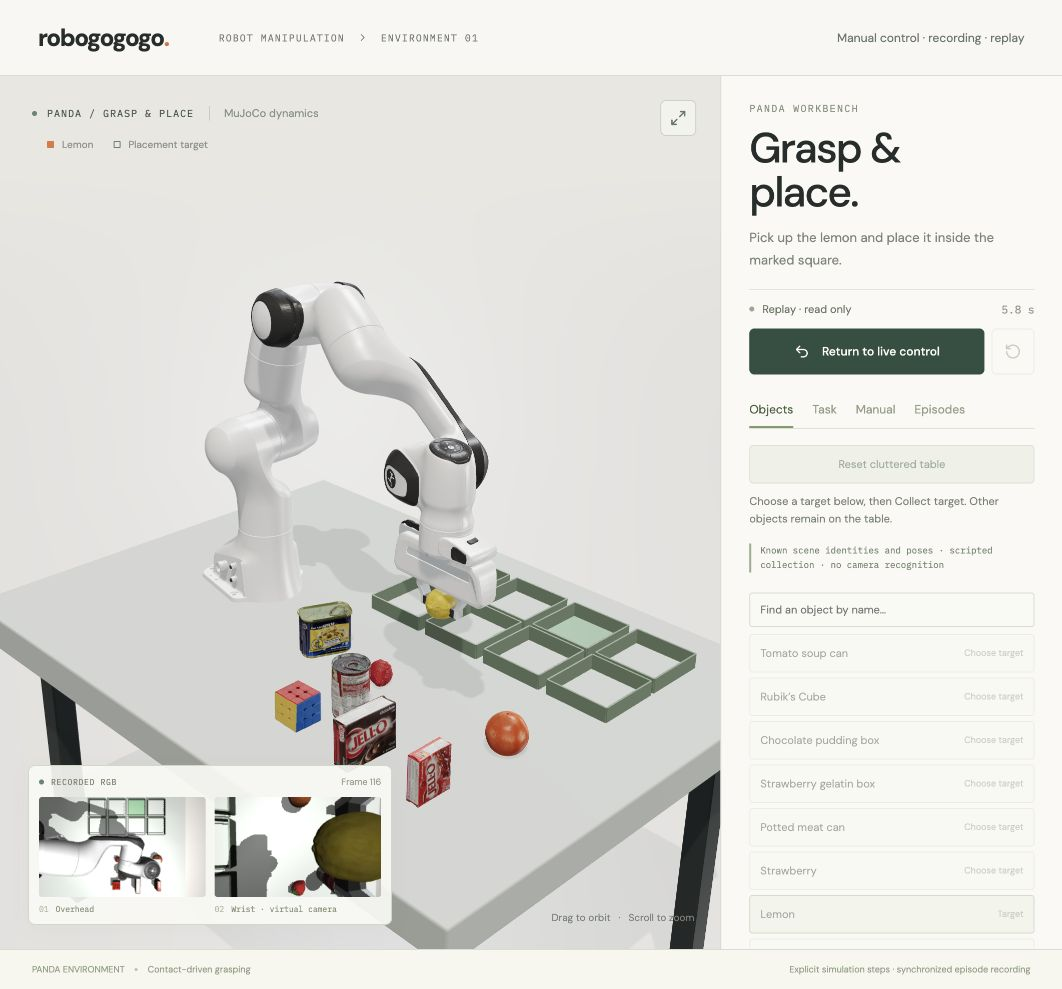
\includegraphics[width=0.86\linewidth]{figures/tabletop.jpg}
\caption{Recorded collection in the eight-object Panda environment. The arm holds the selected lemon while the other scanned objects remain on the table. The lower panels show saved overhead and wrist RGB at the same recorded boundary as the displayed physical state. The reference controller uses known scene poses. Object imagery is from YCB~\cite{ycb,ycbdata}, under CC BY 4.0; the Panda model is from MuJoCo Menagerie~\cite{menagerie}.}
\label{fig:tabletop}
\end{figure}

\section{Related Work}
\subsection{Simulation and Object Assets}
MuJoCo provides articulated-body and contact simulation for control~\cite{mujoco}. Isaac Lab and ManiSkill3 provide broader simulation, sensing, and learning frameworks~\cite{isaaclab,maniskill3}. RoboTwin 2.0 combines an annotated object library, demonstration generation, domain randomization, and bimanual evaluation~\cite{robotwin2}. These systems establish capabilities and comparison settings that extend well beyond the bounded tabletop workflow described here.

The YCB Object and Model Set supplies shared physical objects and digital models for manipulation research~\cite{ycb,ycbdata}. Google Scanned Objects provides a separate, larger collection of scanned household items~\cite{gso}. Robogogogo currently uses eight objects from the Google 16k variants of the YCB releases; these are not downloads from the Google Scanned Objects dataset. The project adds scene assembly and interaction interfaces around these existing assets rather than introducing a new scan dataset.

\subsection{Policies and Demonstration Learning}
Google DeepMind's RT-2 and Gemini Robotics connect visual and language representations to robot behavior~\cite{rt2,geminirobotics}. NVIDIA's GR00T N1 and Physical Intelligence's $\pi_{0.5}$ further motivate interfaces between heterogeneous observations, instructions, and robot actions~\cite{gr00t,pi05}. OpenVLA and Octo offer additional reference points for adapting generalist policies~\cite{openvla,octo}. Their embodiment, image-preprocessing, and action conventions require explicit adaptation before they can control this environment.

Robomimic studies learning from offline demonstrations~\cite{robomimic}, while LIBERO evaluates knowledge transfer across manipulation tasks~\cite{libero}. SIMPLER examines simulated evaluation of real-world policies and the effect of visual and control disparities~\cite{simpler}. These works distinguish an available environment interface from evidence that its data improves learning or that its outcomes predict physical performance. The present work establishes the former workflow and leaves the latter evaluations open.

\subsection{World Models}
World models offer another use for interaction records. DreamerV3 learns a predictive model for imagined control trajectories~\cite{dreamerv3}; Genie studies action-controllable interactive generation from video~\cite{genie}; NVIDIA Cosmos develops world foundation models for physical AI~\cite{cosmos}. For a robot workbench, action-conditioned prediction would require agreement with the robot command, camera geometry, and temporal correspondence of the recorded transition. Robogogogo currently advances explicit MuJoCo dynamics and uses conventional rendering. Its aligned records could support a later world-model study, but no learned simulator or world-model result is included here.

\section{Environment and Object Representation}
\subsection{Robot and Physical Scene}
The current environment uses the official Panda model distributed through MuJoCo Menagerie~\cite{menagerie}. Seven arm joints and two finger coordinates form the robot state. A table supports either one selected object or an eight-object arrangement. Each object has an independent free joint, so contact forces determine its motion throughout grasping, transport, and release. No attachment constraint connects an object to the gripper.

MuJoCo advances at a physics interval of 2\,ms. One environment action holds its command for 25 physics steps, giving a 50\,ms control interval, or 20\,Hz. Manual mode advances only in response to an explicit action. The scripted controller supplies actions on this same interface. Initial scene settling precedes the task clock; a seed determines the bounded variation in starting positions. The multi-object layout uses small position jitter of at most 5\,mm per horizontal axis around a curated arrangement.

The earlier RG Mobile Duo workbench remains a separate Python/JAX environment. Its illustrative mobile dual-arm design, geometric analysis, and hardware-related interfaces are not the embodiment or experimental setting of the Panda task presented here.

\subsection{Scanned Visual Geometry and Collision Models}
Table~\ref{tab:objects} lists the eight scans. Processing preserves metric scale, centers the meshes, and rotates the toy and packages into upright poses. The original texture coordinates are retained, with textures reduced from 4096 to 1024 pixels per side. The can uses a cylindrical collision approximation; the toy and two packages use fitted boxes. Fruit and the meat can use convex mesh collision geometry. These approximations omit small surface features and concavities.

\begin{table}[!htbp]
\centering
\small
\begin{tabular}{lllr}
\toprule
Object & YCB identifier & Collision model & Mass (g)\\
\midrule
Tomato soup can & 005\_tomato\_soup\_can & Cylinder & 350\\
Rubik's Cube & 077\_rubiks\_cube & Box & 90\\
Chocolate pudding box & 008\_pudding\_box & Box & 190\\
Strawberry gelatin box & 009\_gelatin\_box & Box & 90\\
Potted meat can & 010\_potted\_meat\_can & Convex mesh & 170\\
Strawberry & 012\_strawberry & Convex mesh & 20\\
Lemon & 014\_lemon & Convex mesh & 60\\
Orange & 017\_orange & Convex mesh & 140\\
\bottomrule
\end{tabular}
\caption{Curated YCB objects. Masses are assigned simulation parameters, not calibrated measurements. The toy is one rigid body; its faces do not turn. An additional primitive block remains available for the single-object task.}
\label{tab:objects}
\end{table}

Sliding friction is assigned rather than identified from physical trials. The scanned-object configuration uses a gripper tendon servo gain of 300\,N/m within the upstream actuator force limit, accommodating the heavier can. Geometry, friction, mass, servo response, and collision approximation jointly determine the simulated interaction; visual resemblance alone does not establish physical fidelity.

\subsection{Observations and Rendering}
The numerical robot observation has 25 proprioceptive values: nine joint positions, nine velocities, the three-dimensional tool position, and a four-component tool quaternion in XYZW order. The previous eight-dimensional command and task-relative time are also available. Optional overhead and wrist images are RGB arrays of $144\times240$ pixels.

The browser renders MuJoCo poses and scanned textures through Three.js. Native MuJoCo rendering supplies the recorded images and image observations used at the policy boundary. Both views use the model's camera poses and fields of view, but their lighting and material rendering differ. Browser previews should therefore be distinguished from the native images stored in an episode.

\section{Target Collection and Control}
\subsection{Task Definition}
In the multi-object setting, a user selects a named target from the object instances already on the table. Each object has a designated 13\,cm collection cell. Shallow physical walls contain rounded items after release and separate successive destinations. Selecting a new target starts a new task episode while preserving the physical state of the arm, all objects, and previously collected items. Resetting the table instead restores the complete seeded arrangement.

Collection succeeds when the target center is within 6\,cm of the cell center on each horizontal axis and within 8\,mm of its nominal resting height; its translational speed is below 20\,mm/s; the gripper is open beyond 65\,mm with no finger contact; the object was previously lifted by at least 95\,mm; and the tool is more than 120\,mm clear. These conditions must persist for six control steps. Reward is one on success and zero otherwise. Success or an object falling below the workspace terminates the task; the default 800-action limit truncates it. The single-object task uses a 35\,mm horizontal-distance condition around a marked destination instead of a collection cell.

These definitions measure the selected object's transfer and release. They do not impose a quantitative penalty for disturbing another object. The remaining instances continue to respond physically to contacts, and their complete states remain available for later analysis.

\subsection{Manual and Reference Control}
The native action is
\begin{equation}
 a_t=(q^{\star}_{1,t},\ldots,q^{\star}_{7,t},g^{\star}_t)\in\mathbb{R}^{8},
\end{equation}
where arm targets are absolute joint angles in radians and $g^{\star}_t\in[0,0.08]$ is total finger opening in meters. Commands outside the model's joint bounds are rejected. A commanded target is not a measured joint displacement or contact force.

Manual control provides Cartesian tool nudges through inverse kinematics, gripper-opening commands, and single control steps. The reference controller uses smooth joint-target interpolation through approach, descent, grasp, lift, carry, lower, release, and withdrawal phases. It uses known object state to compensate for displacement before grasping and the measured object-to-tool offset before lowering. Bilateral finger contact and retained elevation inform its grasp and transport conditions.

The controller is a bounded scripted procedure rather than a general collision-free planner. It operates on the curated arrangement and can fail on missed contacts, slip, unreachable poses, or an unsettled placement. A failure does not convert into a successful episode through object repositioning or attachment.

\section{Episodes and Policy Integration}
\subsection{Temporal and Scene Correspondence}
An episode with instruction $\ell$ and $H$ actions is represented as
\begin{equation}
 E=\bigl(\ell,\{o_t\}_{t=0}^{H},\{a_t,r_t,d_t,u_t\}_{t=0}^{H-1},\mathcal{M}\bigr),
\end{equation}
where $d_t$ and $u_t$ denote termination and truncation, and $\mathcal{M}$ describes the robot, scene, objects, cameras, and control timing. Transition $t$ associates $o_t$, the command $a_t$, and the resulting $o_{t+1}$. Thus $H$ actions require $H+1$ observation boundaries and, when both cameras are recorded, $2(H+1)$ images.

The record retains the scene's object list, active target, assigned physical properties, model and asset identity, camera geometry, numerical robot and object state, and action source. Manual, scripted, and direct API actions remain distinguishable. Partial and failed runs may be saved. Starting a recording partway through a task preserves the actual starting state and its task-relative time.

Replay restores stored integration states and task bookkeeping for the complete scene. It does not re-execute a policy or assert deterministic action replay across simulator versions. Loading a recorded scene temporarily replaces the displayed environment; leaving replay restores the previous live scene. Target changes and replay therefore have different semantics: the former preserve the live physical scene and begin a new task episode, while the latter display a recorded scene without granting control over it.

\subsection{Policy Observation Boundary}
A policy is expressed as
\begin{equation}
 a_t=\pi_{\theta}(o_t;\ell).
\end{equation}
The policy observation includes proprioception, the previous action, time, and optional overhead/wrist RGB. Scene object lists, object positions, reward, and task-success diagnostics are excluded from this observation. They remain accessible to the environment for bookkeeping and to the scripted reference controller, whose information advantage must be acknowledged in any later comparison.



Both an in-process policy call and an HTTP observation/action interface are available. The latter includes episode identity, a state revision, camera images and geometry, and action bounds and units. A response tied to an outdated revision is rejected rather than applied to a different scene state. This matters when manual interaction or a target change occurs while an external model is computing an action.

A pretrained VLA still needs an adapter for image preprocessing, instruction handling, embodiment, coordinate frames, control rate, and action representation. An end-effector-delta policy, for example, cannot be interpreted directly as eight absolute joint and gripper targets. The interface leaves this adaptation explicit; no learned policy or training procedure is supplied by the current workbench.

\begin{figure}[!h]
\centering
\begin{tikzpicture}[font=\small,box/.style={draw=ink!55,rounded corners,fill=ink!3,align=center,minimum height=13mm,text width=39mm},link/.style={-{Latex[length=2mm]},thick,draw=ink!75}]
\node[box] (browser) {Browser workbench\\Scene / manual controls};
\node[box,right=7mm of browser] (env) {Environment\\MuJoCo / task state};
\node[box,right=7mm of env] (store) {Episode records\\States / actions / RGB};
\node[box,below=9mm of env] (policy) {External policy\\Instruction / RGB / robot state};
\draw[link] (browser) -- (env);
\draw[link] (env) -- (store);
\draw[link] (env) -- node[right,font=\footnotesize]{observations} (policy);
\draw[link] (policy.west) -- ++(-15mm,0) |- (env.south west);
\node[font=\footnotesize,anchor=east] at ([xshift=-18mm,yshift=1mm]policy.west) {actions};
\end{tikzpicture}
\caption{The environment owns physics and task state. A future learned policy receives a restricted observation and returns the same action representation used by the workbench. Recording is independent of which controller supplies the actions.}
\label{fig:architecture}
\end{figure}

\section{Illustrative Demonstration and Scope}
A scripted sequence in the seeded eight-object arrangement collected the soup can, toy, pudding box, gelatin box, meat can, strawberry, lemon, and orange in succession. Each target entered its own collection cell; selecting the next target preserved all physical state. A recorded lemon episode also retained the other seven instances and both camera streams, as illustrated in Figure~\ref{fig:tabletop}.

This sequence demonstrates the intended interaction and recording workflow in one curated arrangement. Controller development used these objects and placements, so the sequence is not a held-out estimate of success probability. It does not establish robustness to occlusion, arbitrary piles, unseen objects, alternative robots, or real-world dynamics. In particular, the target name is resolved through scene identity, and the controller accesses object poses. Language grounding and visual localization remain distinct empirical problems.

The original object sources, approximate contact geometry, and assigned physical parameters further constrain interpretation. The appearance of a familiar product does not imply that its simulated mass, friction, deformation, or contents match a physical counterpart. The current initial arrangement is more structured than an arbitrary cluttered household surface.

\section{Directions for Learning and Evaluation}
A next study can connect an image-conditioned policy to the existing action interface and compare it with the privileged-state reference controller. Such an evaluation should separate target identification from grasp execution, vary instructions and object arrangements, and measure non-target disturbance alongside collection success. Training and evaluation arrangements should be distinct, with repeated seeds and reported failures. Access to object-state metadata must be declared separately from camera-only policy input.

Broader asset and scene import requires additional treatment of collision geometry, scale, articulation, and physical calibration. A scanned room can fuse movable objects with its static background; rendering that room alone does not make its contents independently manipulable. These concerns motivate an incremental progression from individual scans to persistent object scenes before room-scale reconstruction.

These records could support prediction of future images or task-relevant state conditioned on robot commands. Evaluation should address temporal alignment, multi-view consistency, and preservation of collection outcomes. This remains a prospective use of the data; no learned world model is implemented.

\begin{samepage}
\section{Conclusion}
Robogogogo links textured object assets, contact-driven manipulation, persistent tabletop scenes, and aligned episode records. Named-target collection provides a concrete workflow, and the policy boundary supports future VLA integration. Comparative evaluation of learning utility, perceptual generalization, and physical transfer remains future work.

\end{samepage}

\bibliographystyle{plainnat}
\bibliography{references}
\end{document}
